\documentclass[12pt,a4paper]{article}
\usepackage[utf8]{inputenc}
\usepackage[spanish]{babel}
\usepackage{geometry}
\usepackage{amsmath}
\usepackage{amsfonts}
\usepackage{amssymb}
\usepackage{booktabs}
\usepackage{float}
\usepackage{graphicx}

% Configuración de los márgenes
\geometry{top=3cm, bottom=3cm, left=3cm, right=3cm}

% Configuración del título
\title{
    \textbf{Práctica de Laboratorio 1: Paridad}\\
    \large Universidad de Carabobo \\
    Facultad de Ciencias y Tecnología \\
    Departamento de Computación
}
\author{
    \textbf{Integrantes:}\\
    Freddy Ovalle -- C.I: 31.709.650 \\
    Juan Bermúdez -- C.I: 31.608.369
}
\date{Julio de 2026}

\begin{document}

\maketitle


\subsection*{1 ¿Cómo se implementa la recursividad en MIPS32? ¿Qué papel cumple la pila (\$sp)?}
La recursividad en MIPS32 se implementa mediante el uso explícito de la pila, administrada a través del registro \texttt{\$sp} (stack pointer). Cada vez que una función recursiva es llamada, es necesario reservar espacio en la pila para almacenar los registros que podrían ser modificados durante la ejecución, tales como \texttt{\$ra} (return address) y cualquier registro temporal o guardado que esté en uso. 

Antes de realizar una nueva llamada recursiva, se disminuye el valor de \texttt{\$sp} para reservar espacio en memoria y se guardan los registros necesarios. Al finalizar la ejecución de la función, los registros se restauran desde la pila y se incrementa nuevamente \texttt{\$sp} para liberar el espacio reservado. Finalmente, la instrucción \texttt{jr \$ra} permite regresar correctamente al punto desde donde fue llamada la función.

\subsection*{2 ¿Qué riesgos de desbordamiento existen? ¿Cómo mitigarlos?}
\textbf{Desbordamiento de pila} \\
El desbordamiento de pila ocurre cuando se realizan llamadas recursivas excesivas que agotan el espacio de memoria reservado para la pila. Esto puede provocar el bloqueo del programa o comportamientos impredecibles. Generalmente sucede cuando no existe un caso base adecuado o cuando la profundidad de la recursión es demasiado grande.

\textbf{¿Cómo mitigarlo?} \\
Para evitar el desbordamiento de pila se recomienda:
\begin{itemize}
    \item Definir un caso base sólido que garantice la finalización de la recursión.
    \item Verificar cuidadosamente los casos de borde.
    \item Reservar y liberar correctamente el espacio en la pila \texttt{\$sp}.
    \item Evaluar si el problema puede resolverse mediante una solución iterativa cuando la profundidad de recursión sea considerable.
\end{itemize}

\subsection*{3 ¿Qué diferencias encontraste entre una implementación iterativa y una recursiva en cuanto al uso de memoria y registros?}
Para resolver el algoritmo de paridad, el método iterativo se consolida como la opción más directa y ligera en cuanto al uso de hardware. Debido a que no necesita almacenar datos contextuales en la pila en cada ciclo, mantiene un uso mínimo de los registros internos y no satura la memoria principal.

Por su parte, la solución recursiva requiere una gestión mucho más meticulosa de la arquitectura, ya que se ve obligada a abrir espacio nuevo en la pila por cada nivel de ejecución. A pesar de que el código recursivo posee un diseño teórico más refinado, este beneficio estético se ve opacado por un incremento lineal en el consumo de memoria, haciendo que su rendimiento sea inferior al del esquema iterativo.

\subsection*{4 ¿Qué diferencias encontraste entre los ejemplos académicos del libro y un ejercicio completo y operativo en MIPS32?}
Los ejemplos del libro muestran casos aislados del funcionamiento de instrucciones y de la pila, omitiendo a veces la inicialización de ciertos registros; además, no manejan datos de entrada ni salida con \texttt{syscall} sino directamente se enfocan en operarlos para mostrar la ejecución paso a paso. Por otra parte, en un ejercicio completo debemos inicializar los registros involucrados, se hace uso de la entrada y salida y se implementa los casos mostrados en el libro pero en conjunto.

\subsection*{5 Ejecucion paso a paso en MARS}
Supongamos que la entrada por pantalla es igual a 7.

\textbf{Inicio del Programa (Entrada de Datos)}
\begin{itemize}
    \item \textbf{Pasos 1 a 3:} Se configura \texttt{\$v0} con el código 4, se apunta \texttt{\$a0} al texto ``ingrese un numero '' y la instrucción \texttt{syscall} lo muestra en pantalla.
    \item \textbf{Pasos 4 y 5:} Se cambia \texttt{\$v0} a 5 y con \texttt{syscall} el programa lee el número ingresado ( 7 ).
    \item \textbf{Paso 6:} Se transfiere el valor leído al registro guardado: \texttt{\$s0} = 7.
\end{itemize}

\textbf{Inicialización de Variables}
\begin{itemize}
    \item \textbf{Paso 7:} El registro que almacena el resultado alternante se inicializa en cero: \texttt{\$t0} = 0 (0 significa par, 1 significa impar).
    \item \textbf{Paso 8:} El contador de vueltas del bucle se inicializa en cero: \texttt{\$t1} = 0.
\end{itemize}

\textbf{Ejecución del Bucle (Ciclo for)} \\
El programa evalúa en la etiqueta \texttt{for} si el contador \texttt{\$t1} ha alcanzado el límite \texttt{\$s0} (7). Si no se cumple, entra al ciclo, carga la constante 1 en \texttt{\$t2}, calcula el nuevo estado de la paridad restando (\texttt{\$t0} = 1 - \texttt{\$t0}) e incrementa el contador en 1 antes de saltar de nuevo con \texttt{j for}.

\begin{itemize}
    \item \textbf{Vuelta 1:} Evalúa 0 == 7 (Falso). Alterna: \texttt{\$t0} = 1 - 0 = 1. Incrementa contador: \texttt{\$t1} = 1.
    \item \textbf{Vuelta 2:} Evalúa 1 == 7 (Falso). Alterna: \texttt{\$t0} = 1 - 1 = 0. Incrementa contador: \texttt{\$t1} = 2.
    \item \textbf{Vuelta 3:} Evalúa 2 == 7 (Falso). Alterna: \texttt{\$t0} = 1 - 0 = 1. Incrementa contador: \texttt{\$t1} = 3.
    \item \textbf{Vuelta 4:} Evalúa 3 == 7 (Falso). Alterna: \texttt{\$t0} = 1 - 1 = 0. Incrementa contador: \texttt{\$t1} = 4.
    \item \textbf{Vuelta 5:} Evalúa 4 == 7 (Falso). Alterna: \texttt{\$t0} = 1 - 0 = 1. Incrementa contador: \texttt{\$t1} = 5.
    \item \textbf{Vuelta 6:} Evalúa 5 == 7 (Falso). Alterna: \texttt{\$t0} = 1 - 1 = 0. Incrementa contador: \texttt{\$t1} = 6.
    \item \textbf{Vuelta 7:} Evalúa 6 == 7 (Falso). Alterna: \texttt{\$t0} = 1 - 0 = 1. Incrementa contador: \texttt{\$t1} = 7.
\end{itemize}

\textbf{Salida e Impresión de Resultados}
\begin{itemize}
    \item \textbf{Evaluación final:} Al volver a subir, la instrucción \texttt{beq \$t1, \$s0, imprimir} comprueba la condición 7 == 7. Al ser Verdadero, el programa rompe el bucle y salta a la etiqueta imprimir.
    \item \textbf{Impresión del texto:} Se configura \texttt{\$v0} en 4, se carga en \texttt{\$a0} la dirección de ``el resultado es: '' y se ejecuta \texttt{syscall}.
    \item \textbf{Impresión del valor:} Se copia el resultado final obtenido (\texttt{\$t0} = 1) al registro \texttt{\$a0}, se configura \texttt{\$v0} en 1 (imprimir entero) y \texttt{syscall} muestra el 1 en la consola, confirmando que el número es impar.
    \item \textbf{Fin del programa:} Se carga el código de término 10 en \texttt{\$v0} y se ejecuta el último \texttt{syscall} para cerrar el simulador MARS de forma segura.
\end{itemize}

\subsection*{6 justificar la elección del enfoque (iterativo o recursivo) según eficiencia y claridad en MIPS.}
Tomando en cuenta los puntos detallamos anteriormente, escogimos el enfoque iterativo para el algoritmo de paridad, ya que nos ofrece mayor eficiencia en cuanto a espacio en memoria al evitar por completo la latencia que introduce el acceso a la memoria RAM (operaciones de carga y almacenamiento), resolviendo todo mediante registros internos muy rápidos. Mientras que el código recursivo necesita realizar múltiples operaciones en la pila para procesar una entrada baja como $n=7$, la versión por ciclos despacha el problema en apenas 54 instrucciones bajo la misma entrada.

\subsection*{7 Análisis y Discusión de los resultados}
Al evaluar el desempeño del método iterativo, se evidencia que su comportamiento responde a un orden $O(n)$, lo que genera tiempos de respuesta excesivos ante entradas de gran magnitud. Esta limitación pone de manifiesto que la estrategia correcta para este problema requiere el uso de la instrucción \texttt{andi}, la cual optimiza el algoritmo a una complejidad $O(1)$ al validar únicamente el último bit del registro.

Asimismo, esta lógica por ciclos resulta incompatible con números negativos, puesto que el bucle interrumpe su marcha en el momento en que la variable cumple la condición $n \le 1$. Como contraparte experimental, las pruebas de ejecución ejecutadas en MARS para un valor de $n = 7$ reflejaron que el enfoque iterativo requiere un total de 54 instrucciones para resolver el problema.

\begin{figure}[H]
    \centering
    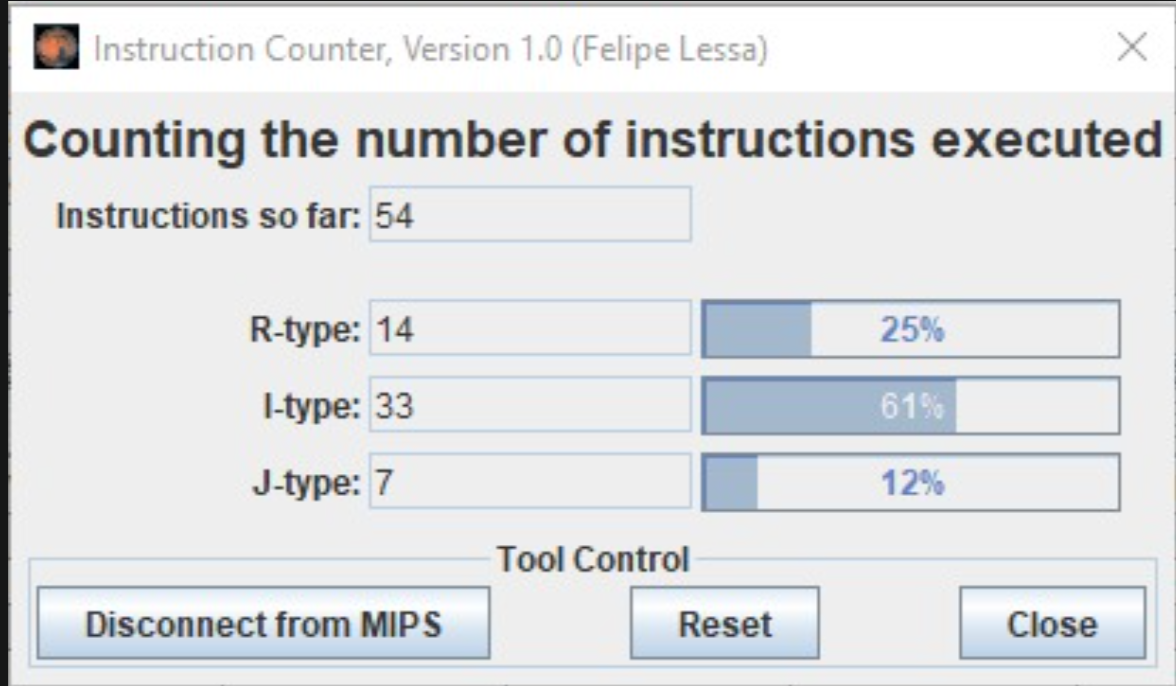
\includegraphics[width=0.5\linewidth]{iterativo.png}
    \caption{Contador de Instrucciones de MARS – Enfoque Iterativo}
    \label{fig:placeholder}
\end{figure}

\begin{figure}[H]
    \centering
    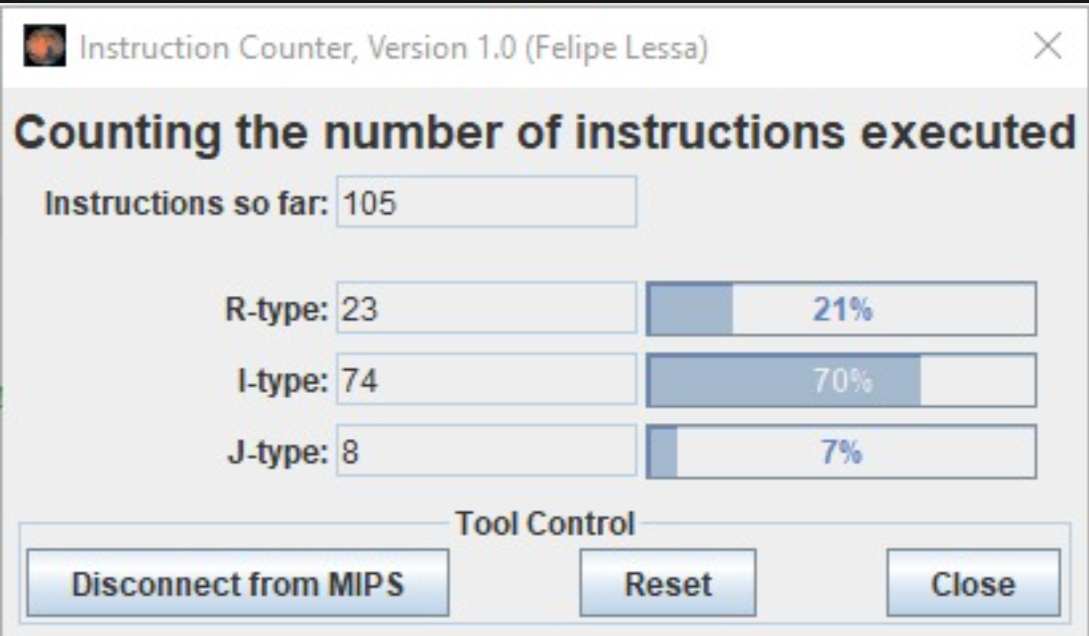
\includegraphics[width=0.5\linewidth]{recursivo.png}
    \caption{Contador de Instrucciones de MARS – Enfoque Recursivo}
    \label{fig:placeholder}
\end{figure}

\end{document}